% Paste this entire file into Overleaf main.tex
% Ensure Graphs/ folder contains choropleth_htm_2017Q1.png through choropleth_htm_2018Q4.png

\documentclass{beamer}
\usetheme{Madrid}
\usecolortheme{default}
\usepackage{amsmath,amssymb}
\usepackage{booktabs}
\usepackage{graphicx}

\sloppy

\title{Hand-to-Mouth Agent Classification for Brazil}
\subtitle{Kaplan--Violante--Weidner (2014) applied to POF 2017--18 \& PNADC}
\author{}
\institute{}
\date{}

\begin{document}

\begin{frame}
  \titlepage
\end{frame}

\begin{frame}{H2M Classification}
  \textbf{Goal:} Classify Brazilian households into three agent types (Kaplan, Violante \& Weidner 2014)
  \begin{itemize}
    \item \textbf{PH2M} (Poor HtM) --- low liquid, low illiquid assets
    \item \textbf{WH2M} (Wealthy HtM) --- low liquid, significant illiquid assets
    \item \textbf{Ricardian} --- sufficient liquid buffer to smooth consumption
  \end{itemize}
  \vspace{0.5em}
  Type shares estimated in POF $\to$ transferred to PNADC via bin-matching \& Monte Carlo $\Rightarrow$ state$\times$quarter panel for HANK.
  \vspace{0.5em}
  \textbf{Literature targets (Brazil):} Carvalho \& Zilberman (2022); De Souza (2023) --- PH2M 20--28\%, WH2M 12--18\%, Ricardian 55--65\%, Total HtM 35--45\%.
\end{frame}

\section{Data \& Pipeline}

\begin{frame}{Data Sources}
  \begin{table}
    \scriptsize
    \resizebox{\textwidth}{!}{%
    \begin{tabular}{lllll}
      \toprule
      \textbf{Survey} & \textbf{Period} & \textbf{Sample} & \textbf{Format} & \textbf{Key variables} \\
      \midrule
      POF 2017--18 & Jul 2017--Jul 2018 & $\sim$140k (age $\geq$ 15) & Fixed-width (5 tbl) & Income, assets (imputed), expenditure, weights \\
      PNADC & 2017 Q1--2018 Q4 (8 qtrs) & varies & CSV (test5/6/7) & Demographics, income, employment, weights \\
      \bottomrule
    \end{tabular}%
    }
  \end{table}
\end{frame}

\begin{frame}{POF Table Structure}
  POF: five fixed-width text files (column positions from Excel data dictionary)
  \begin{table}
    \tiny
    \resizebox{\textwidth}{!}{%
    \begin{tabular}{ll}
      \toprule
      \textbf{File} & \textbf{Key columns} \\
      \midrule
      \texttt{DOMICILIO.txt} & COD\_UPA, NUM\_DOM, UF, PESO\_FINAL \\
      \texttt{MORADOR.txt} & V0403 (age), V0404 (sex), NIVEL\_INSTRUCAO, RENDA\_TOTAL \\
      \texttt{RENDIMENTO\_TRABALHO.txt} & V8500\_DEFLA (deflated labour inc.), V5302/V5303 (formality) \\
      \texttt{OUTROS\_RENDIMENTOS.txt} & QUADRO 55=pension, 56=govt transfers, 57=financial income \\
      \texttt{ALUGUEL\_ESTIMADO.txt} & V8000\_DEFLA (estimated rent $\to$ real estate proxy) \\
      \bottomrule
    \end{tabular}%
    }
  \end{table}
\end{frame}

\begin{frame}{Pipeline Architecture}
  \begin{enumerate}
    \item POF: Load \& merge 5 tables $\rightarrow$ classify each person
    \item POF: 6D bins $\rightarrow$ weighted shares (Dirichlet $\alpha=0.1$)
    \item PNADC: Same 6D bins $\rightarrow$ left-merge POF shares
    \item PNADC: Monte Carlo type draw (seed=42)
    \item PNADC: Aggregate to state$\times$quarter shares
    \item PNADC: Generate choropleth maps per quarter
  \end{enumerate}
\end{frame}

\section{Classification Methodology}

\begin{frame}{Zero-Financial-Income Problem}
  Only \textbf{8\%} of POF individuals report financial income (QUADRO 57).
  \vspace{0.5em}
  Naive: $\text{liquid} = (\text{fin.\ inc.} \times 12)/\text{SELIC}$ $\Rightarrow$ 92\% get zero, all HtM.
  \vspace{0.5em}
  Grid search (864 combinations): best achievable total HtM $\approx$ 91.5\% vs target $\approx$ 40\%.
\end{frame}

\begin{frame}{Augmented Liquid Asset Imputation}
  \small
  \[
  \text{liquid} = \underbrace{\frac{\text{fin.\ inc.} \times 12}{\text{SELIC}}}_{\text{fin.}} + \underbrace{\text{pen.} \times 1}_{\text{buf.}} + \underbrace{\max(0,\, \text{R\_T} - 12\times\text{inc.}) \times 0.5}_{\text{savings}}
  \]
  Savings proxy zeroed for Bolsa Família recipients (QUADRO 56 $>$ 0).
\end{frame}

\begin{frame}{Two-Threshold Classification Rule}
  \small
  \[
  \text{type} = \begin{cases}
    \text{Ricardian} & \text{liquid} > \lambda \\
    \text{WH2M} & \text{liquid} \leq \lambda,\ \text{illiquid} \geq \mu \\
    \text{PH2M} & \text{else}
  \end{cases}
  \]
  $\lambda=0.50$, $\mu=3$ (monthly income).
\end{frame}

\begin{frame}{Calibrated Parameters}
  \begin{table}
    \scriptsize
    \resizebox{\textwidth}{!}{%
    \begin{tabular}{llp{5.2cm}}
      \toprule
      \textbf{Parameter} & \textbf{Value} & \textbf{Description} \\
      \midrule
      SELIC\_RATE & 0.09 & Annual rate for capitalising financial income \\
      LIQUID\_THRESH & 0.50 & Liquid assets / monthly income threshold ($\lambda$) \\
      ILLIQUID\_MULT & 3 & Illiquid assets / monthly income threshold ($\mu$) \\
      PENSION\_MULT & 1 & Months of pension held as liquid buffer \\
      SAVINGS\_FRAC & 0.50 & Fraction of income surplus treated as savings \\
      POVERTY\_LINE & R\$170 & BRL/month per capita (Bolsa Família line, diagnostic) \\
      \bottomrule
    \end{tabular}%
    }
  \end{table}
\end{frame}

\section{Bin Matching}

\begin{frame}{Six Bin Dimensions}
  \scriptsize
  \resizebox{\textwidth}{!}{%
  \begin{tabular}{lll}
    \toprule
    \textbf{Dimension} & \textbf{Values} & \textbf{Notes} \\
    \midrule
    macro\_region & North, NE, SE, South, Central\_West & UF $\to$ region cut \\
    age\_group & 15--24, ..., 65+ (6-way emp.; 3-way inact.) & Coarser for inactive \\
    gender & male, female & POF V0404; PNADC V2007 \\
    education\_group & no\_ed., primary, secondary, tertiary & POF NIVEL\_INSTRUCAO; PNADC VD3004 \\
    inc\_band & B1--B5 (BRL [170, 700, 2k, 4k]); no\_income inact. & Absolute bands, same in both \\
    labour\_3way & employed, unemployed, inactive & formal+inf+SE $\to$ employed \\
    \bottomrule
  \end{tabular}%
  }
\end{frame}

\begin{frame}{Mismatch Problem}
  Initial 6D bin scheme: \textbf{60.2\% match} (355k of 893k PNADC individuals unmatched).
  \vspace{0.5em}
  \textbf{Root causes:}
  \begin{enumerate}
    \item Labour-status label mismatch: POF 3-way vs PNADC 5-way (formal/informal/SE/unemp/inactive). Dropping labour alone $\to$ 99.8\% match.
    \item Relative quintiles: Q1 in POF $\neq$ Q1 in PNADC; 100\% of Q1$\times$informal unmatched.
  \end{enumerate}
  \vspace{0.3em}
  \scriptsize \textit{Illustrative; actual values depend on PNADC panels loaded.}
\end{frame}

\begin{frame}{Mismatch Fix --- Before/After}
  \begin{table}
    \scriptsize
    \resizebox{\textwidth}{!}{%
    \begin{tabular}{lll}
      \toprule
      \textbf{Dimension} & \textbf{Before} & \textbf{After} \\
      \midrule
      labour\_status & 5-way (formal/informal/SE/unemp/inact.) & 3-way (formal+inf+SE $\to$ employed) \\
      income\_band & Relative per-survey quintile (Q1--Q5) & Absolute BRL bands [170, 700, 2k, 4k] \\
      inactive income & Quintile assigned normally & Fixed \texttt{no\_income} \\
      age\_group (inactive) & 6-way for all & 3-way (15--34, 35--54, 55+) \\
      \bottomrule
    \end{tabular}%
    }
  \end{table}
\end{frame}

\begin{frame}{Strategy Comparison}
  \begin{table}
    \scriptsize
    \resizebox{\textwidth}{!}{%
    \begin{tabular}{llll}
      \toprule
      \textbf{Strategy} & \textbf{POF bins} & \textbf{Match rate} & \textbf{Trade-off} \\
      \midrule
      A: Original (relative quintile + 5-way labour) & 3,102 & 60.2\% & Baseline --- too many unmatched \\
      D: Drop labour entirely (5D) & 1,180 & 99.8\% & Loses employment heterogeneity \\
      G: 3-way labour + conditional absolute bands & 1,361 & $\sim$77\% & Best balance; chosen \\
      I: Drop labour, conditional absolute bands & 1,361 & 99.9\% & Near-perfect match, no labour dim. \\
      \bottomrule
    \end{tabular}%
    }
  \end{table}
  Strategy G: 1,361 bins; only 1 small bin ($<$30 weighted obs).
\end{frame}

\section{Validation}

\begin{frame}{National Validation}
  \begin{table}
    \scriptsize
    \resizebox{\textwidth}{!}{%
    \begin{tabular}{lcccc}
      \toprule
      \textbf{Stage} & \textbf{PH2M} & \textbf{WH2M} & \textbf{Ricardian} & \textbf{Total HtM} \\
      \midrule
      1. POF Classification & 21.5\% & 19.3\% & 59.2\% & 40.8\% \\
      3. PNADC Post-Merge & 25.0\% & 28.0\% & 47.0\% & 53.0\% \\
      4. PNADC Post-MC & 24.9\% & 28.0\% & 47.0\% & 53.0\% \\
      Literature target & 20--28\% & 12--18\% & 55--65\% & 35--45\% \\
      \bottomrule
    \end{tabular}%
    }
  \end{table}
  Monte Carlo realised shares track expected within $\sim$0.1 pp.
  \vspace{0.5em}
  \begin{block}{Warning}
    PNADC WH2M (28\%) elevated vs POF (19.3\%) and literature (12--18\%). Driven by 22.7\% unmatched rows falling back to national averages, and inactive individuals matched to high-illiquid POF bins.
  \end{block}
\end{frame}

\section{Regional Results}

\begin{frame}{Key Regional Patterns}
  \begin{itemize}
    \item \textbf{PH2M} highest in \textbf{Northeast} (e.g.\ Maranhão 26.4\%) --- poverty, low financial inclusion
    \item \textbf{WH2M} highest in \textbf{North} (e.g.\ Amazonas 22.4\%) --- land/housing but low liquid access
    \item \textbf{Ricardian} highest in \textbf{Southeast/South} (e.g.\ São Paulo 64.5\%) --- financial development, formal labour
    \item \textbf{Total HtM}: clear North/Northeast vs South/Southeast gradient --- heterogeneity for HANK
  \end{itemize}
\end{frame}

\begin{frame}{Choropleth Maps --- 2017 Q1}
  \vspace{-0.5em}
  \begin{center}
    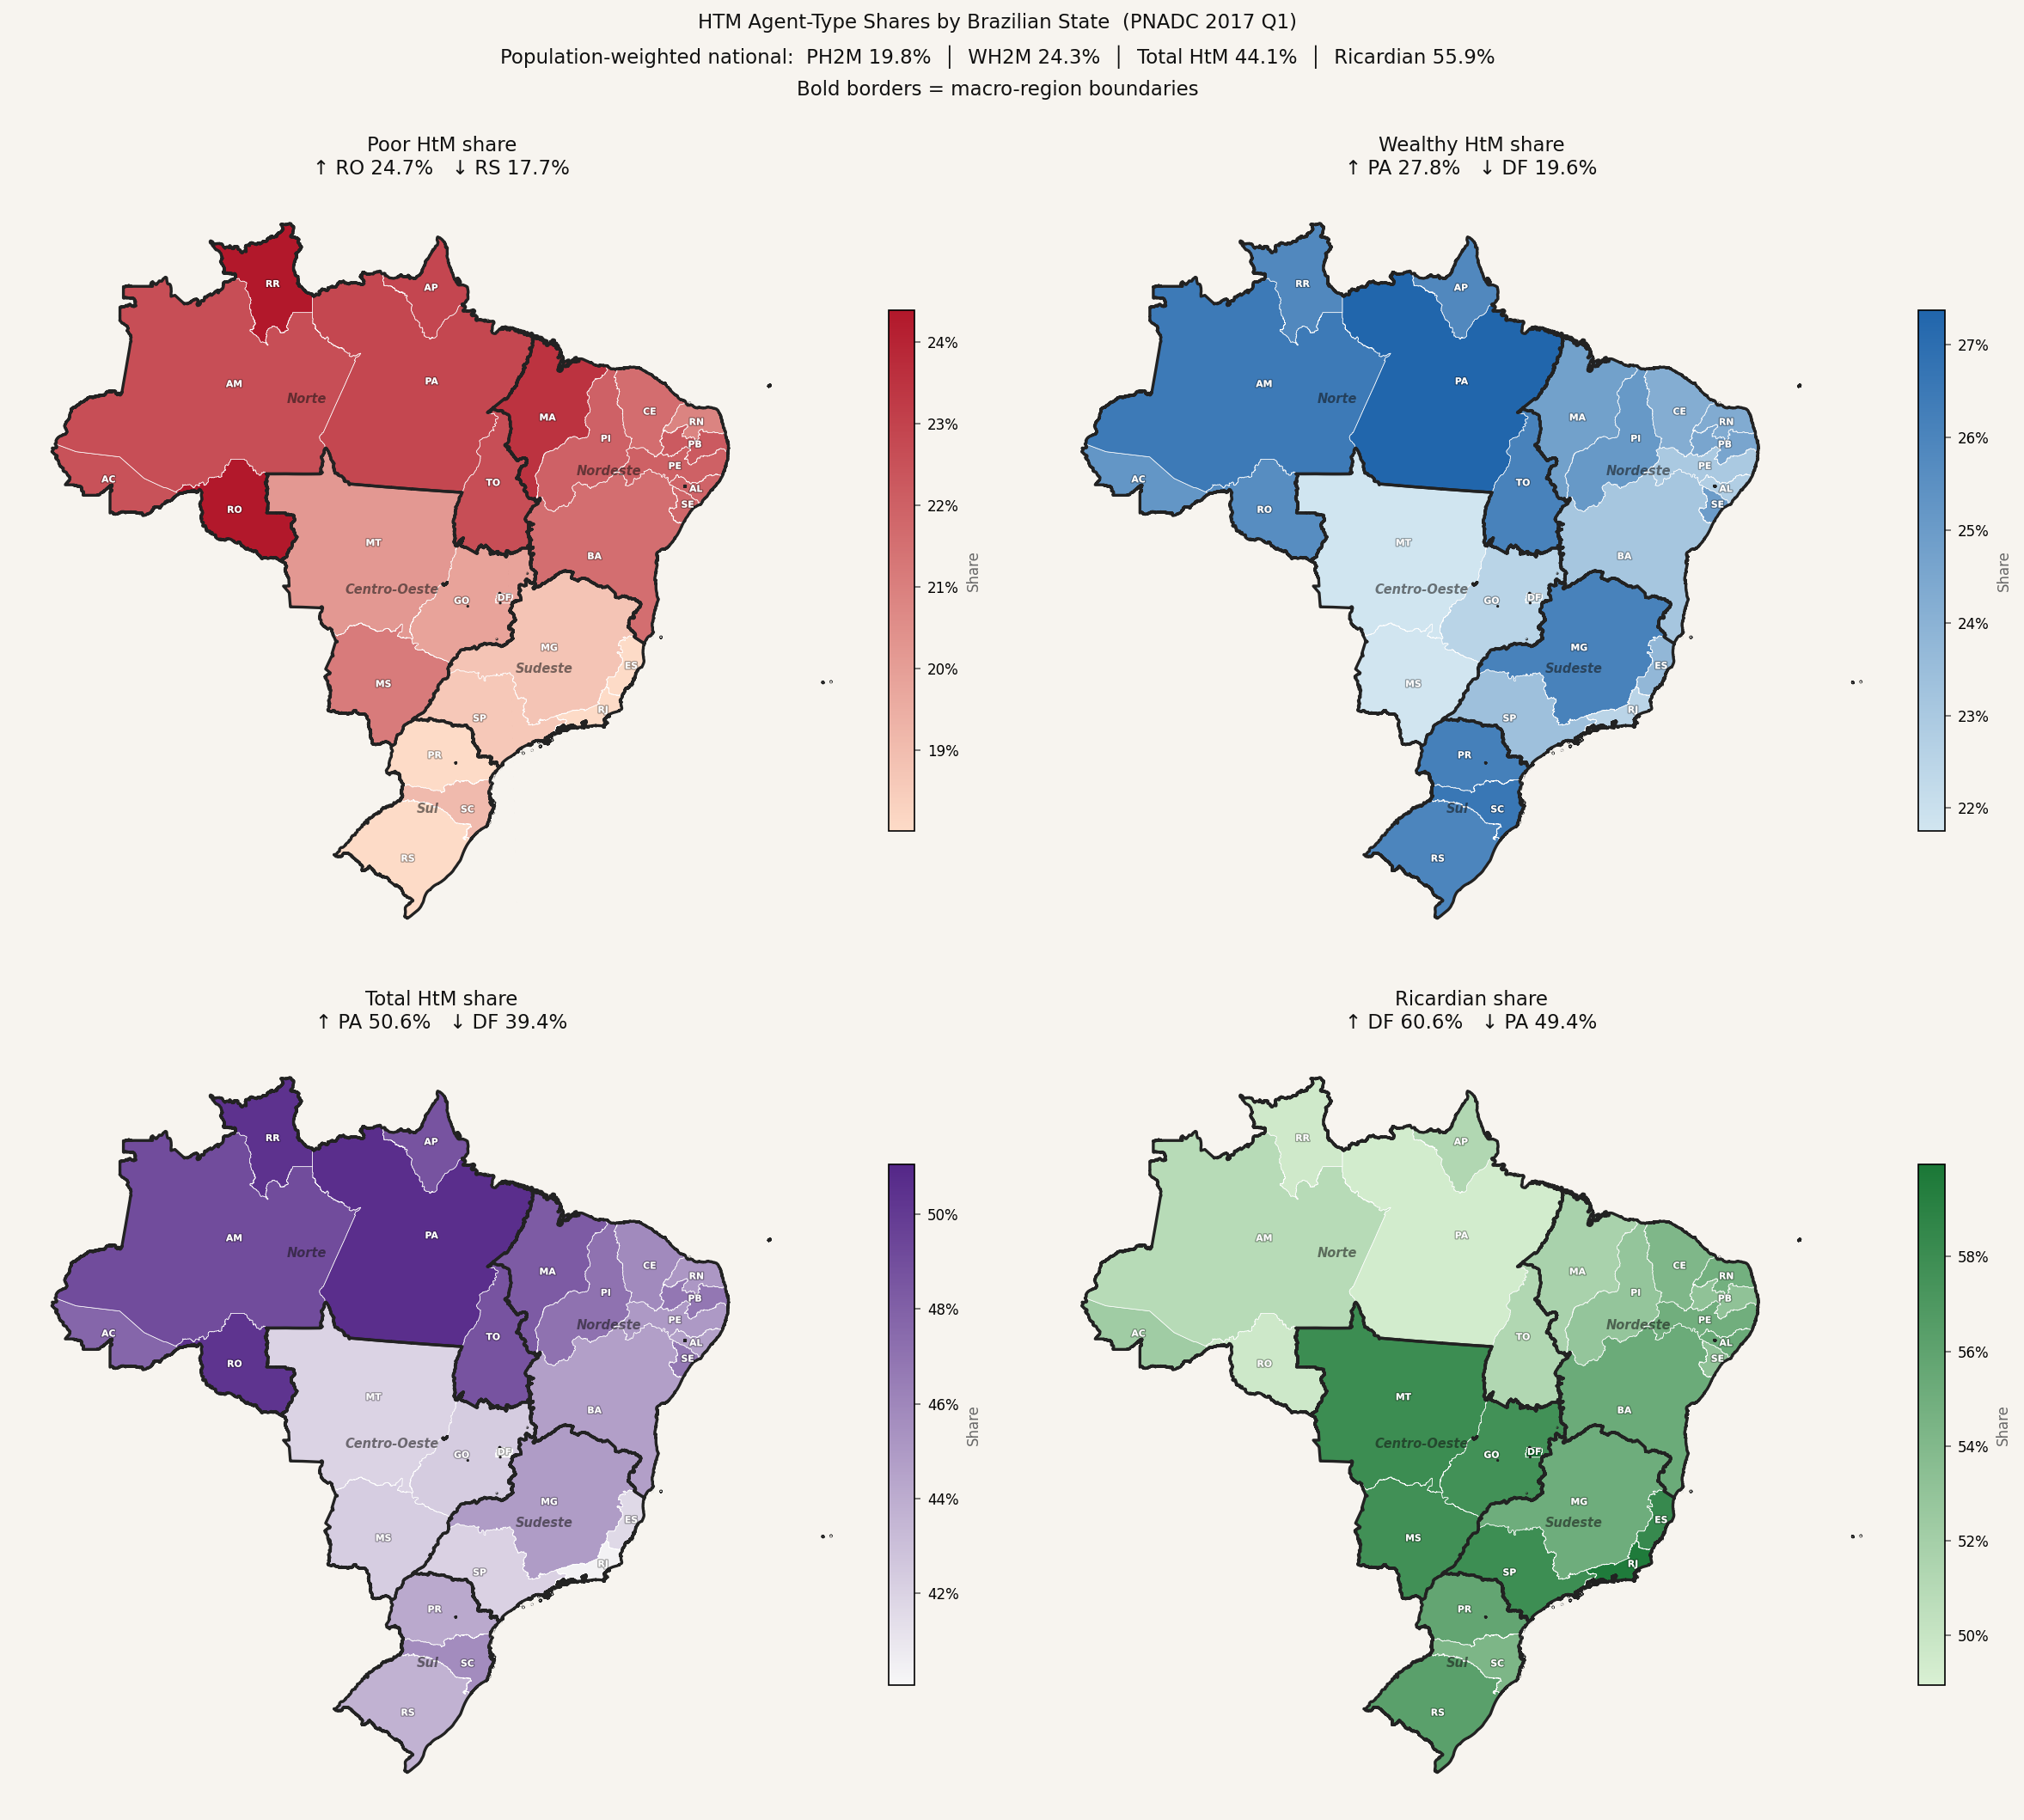
\includegraphics[height=0.75\textheight,keepaspectratio]{Graphs/choropleth_htm_2017Q1.png}
  \end{center}
\end{frame}

\begin{frame}{Choropleth Maps --- 2017 Q2}
  \vspace{-0.5em}
  \begin{center}
    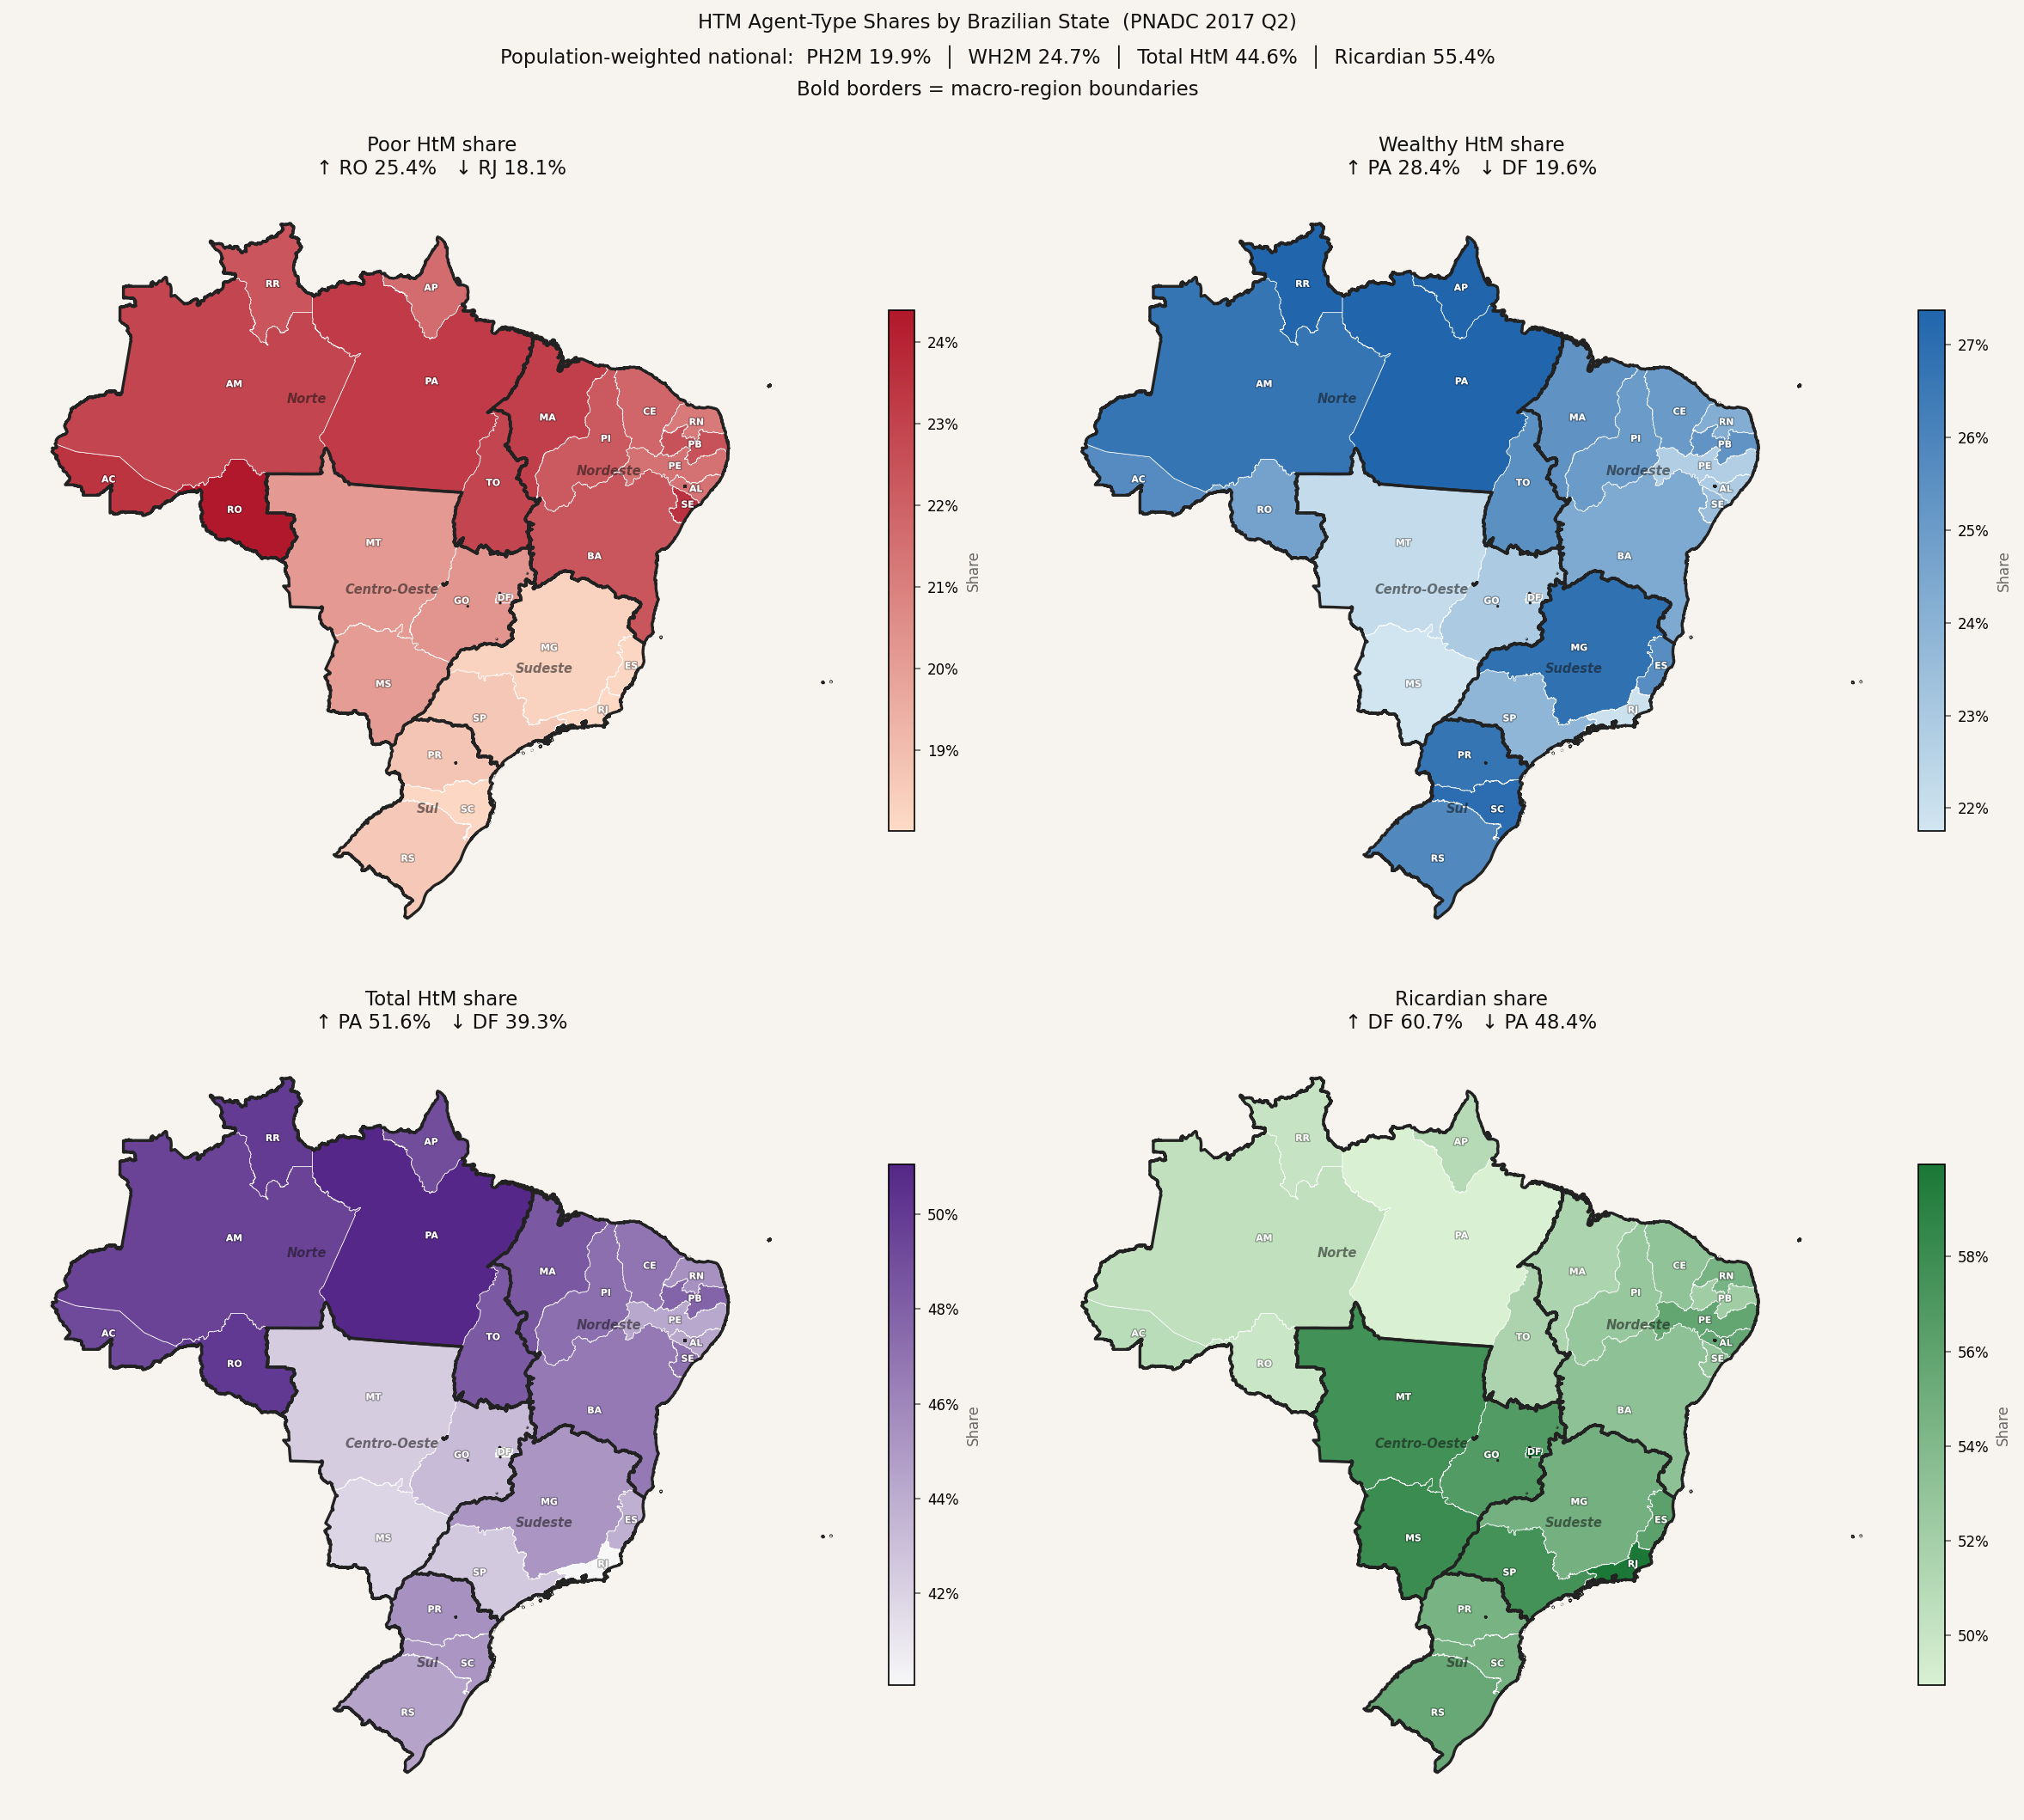
\includegraphics[height=0.75\textheight,keepaspectratio]{Graphs/choropleth_htm_2017Q2.png}
  \end{center}
\end{frame}

\begin{frame}{Choropleth Maps --- 2017 Q3}
  \vspace{-0.5em}
  \begin{center}
    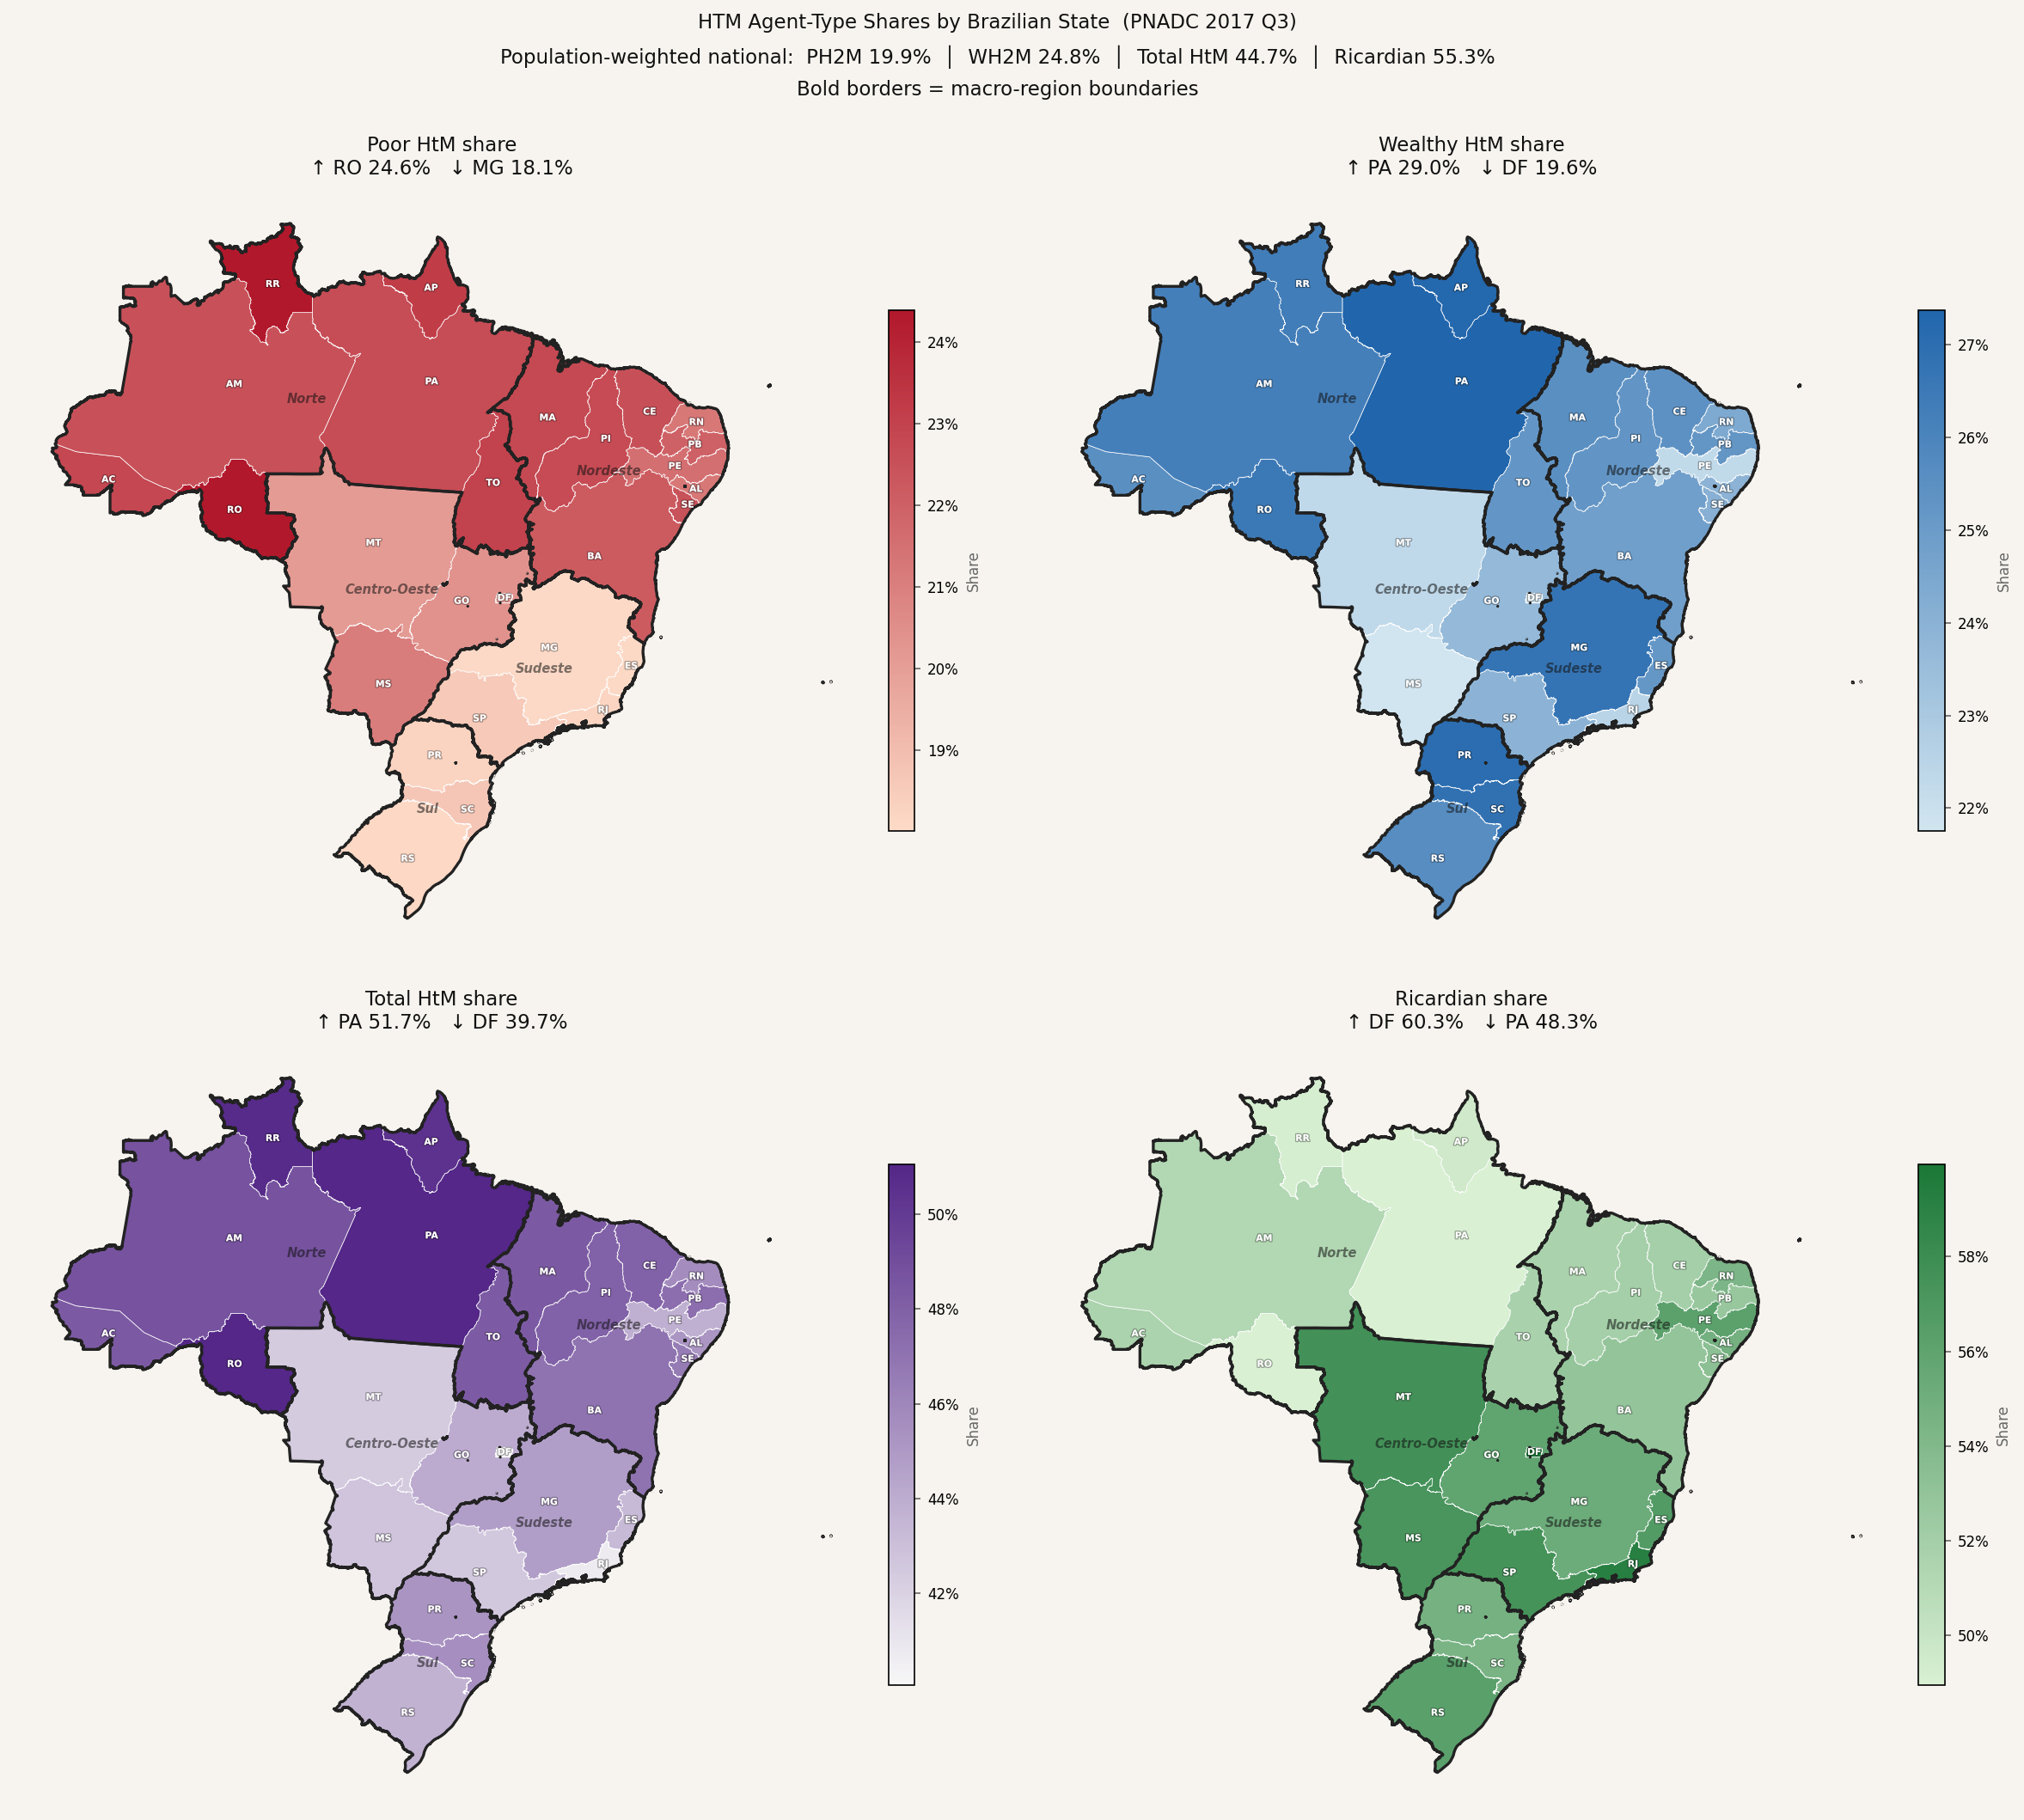
\includegraphics[height=0.75\textheight,keepaspectratio]{Graphs/choropleth_htm_2017Q3.png}
  \end{center}
\end{frame}
\begin{frame}{Choropleth Maps --- 2017 Q4}
  \vspace{-0.5em}
  \begin{center}
    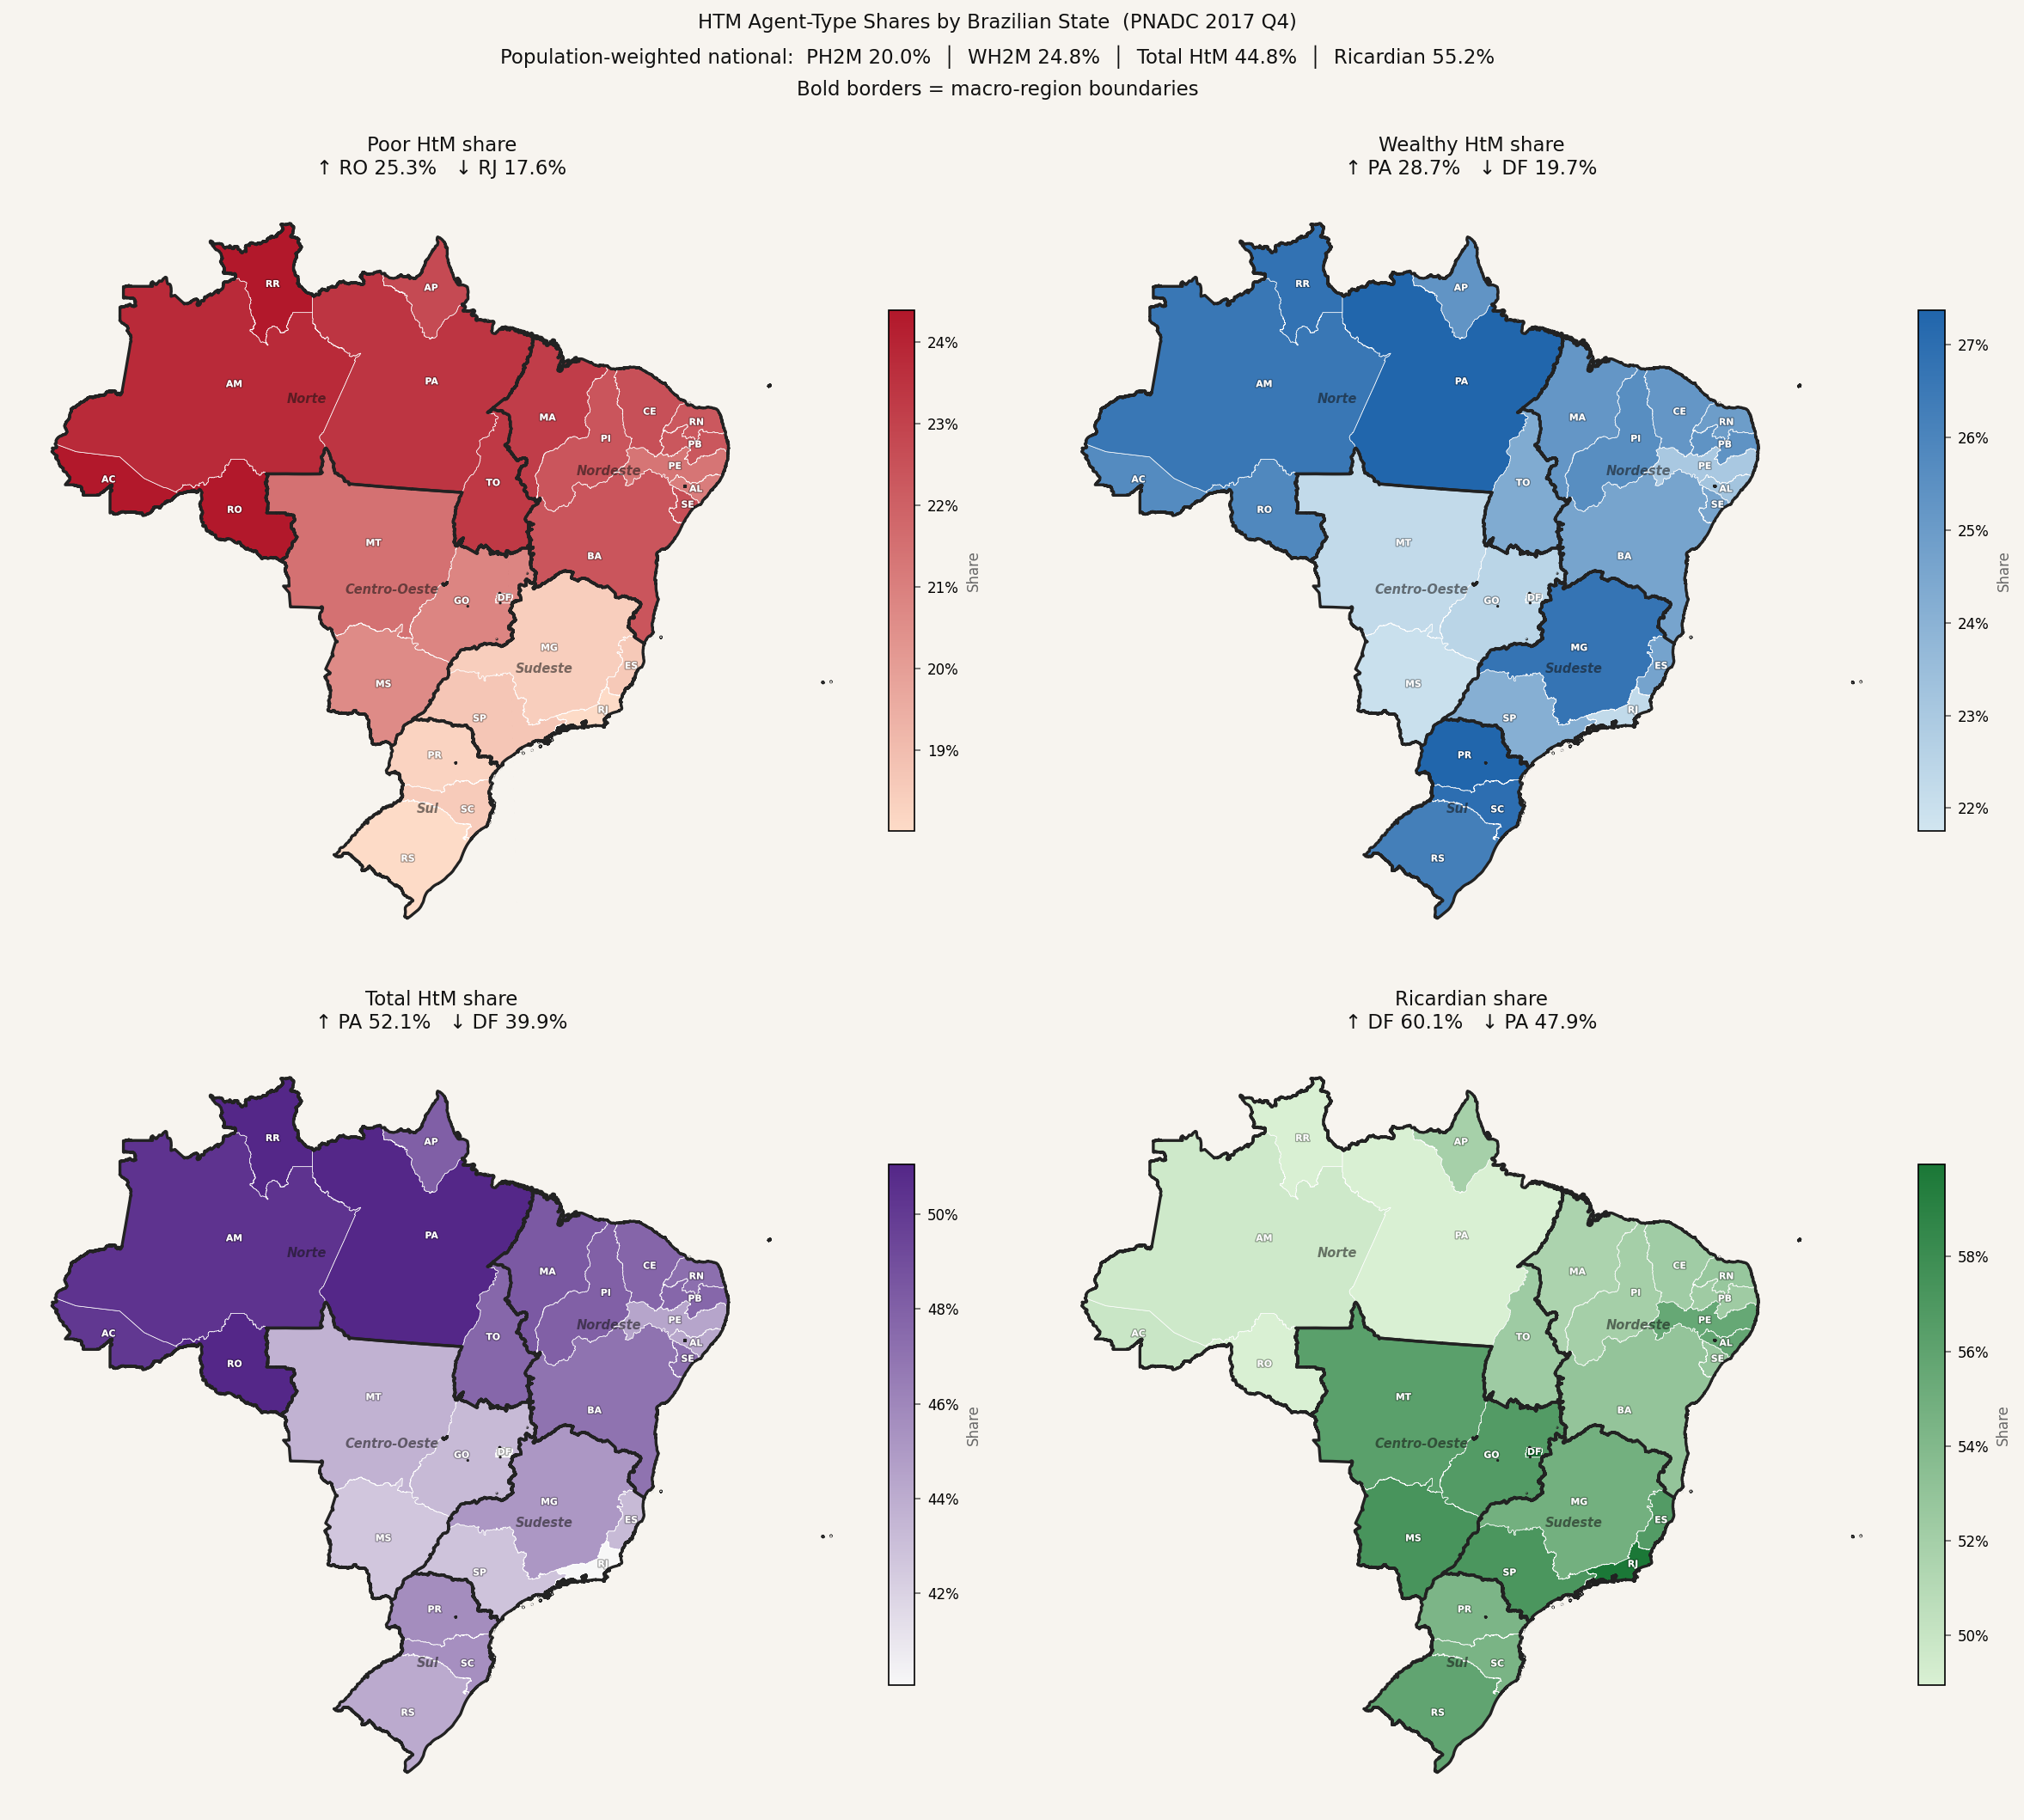
\includegraphics[height=0.75\textheight,keepaspectratio]{Graphs/choropleth_htm_2017Q4.png}
  \end{center}
\end{frame}
\begin{frame}{Choropleth Maps --- 2018 Q1}
  \vspace{-0.5em}
  \begin{center}
    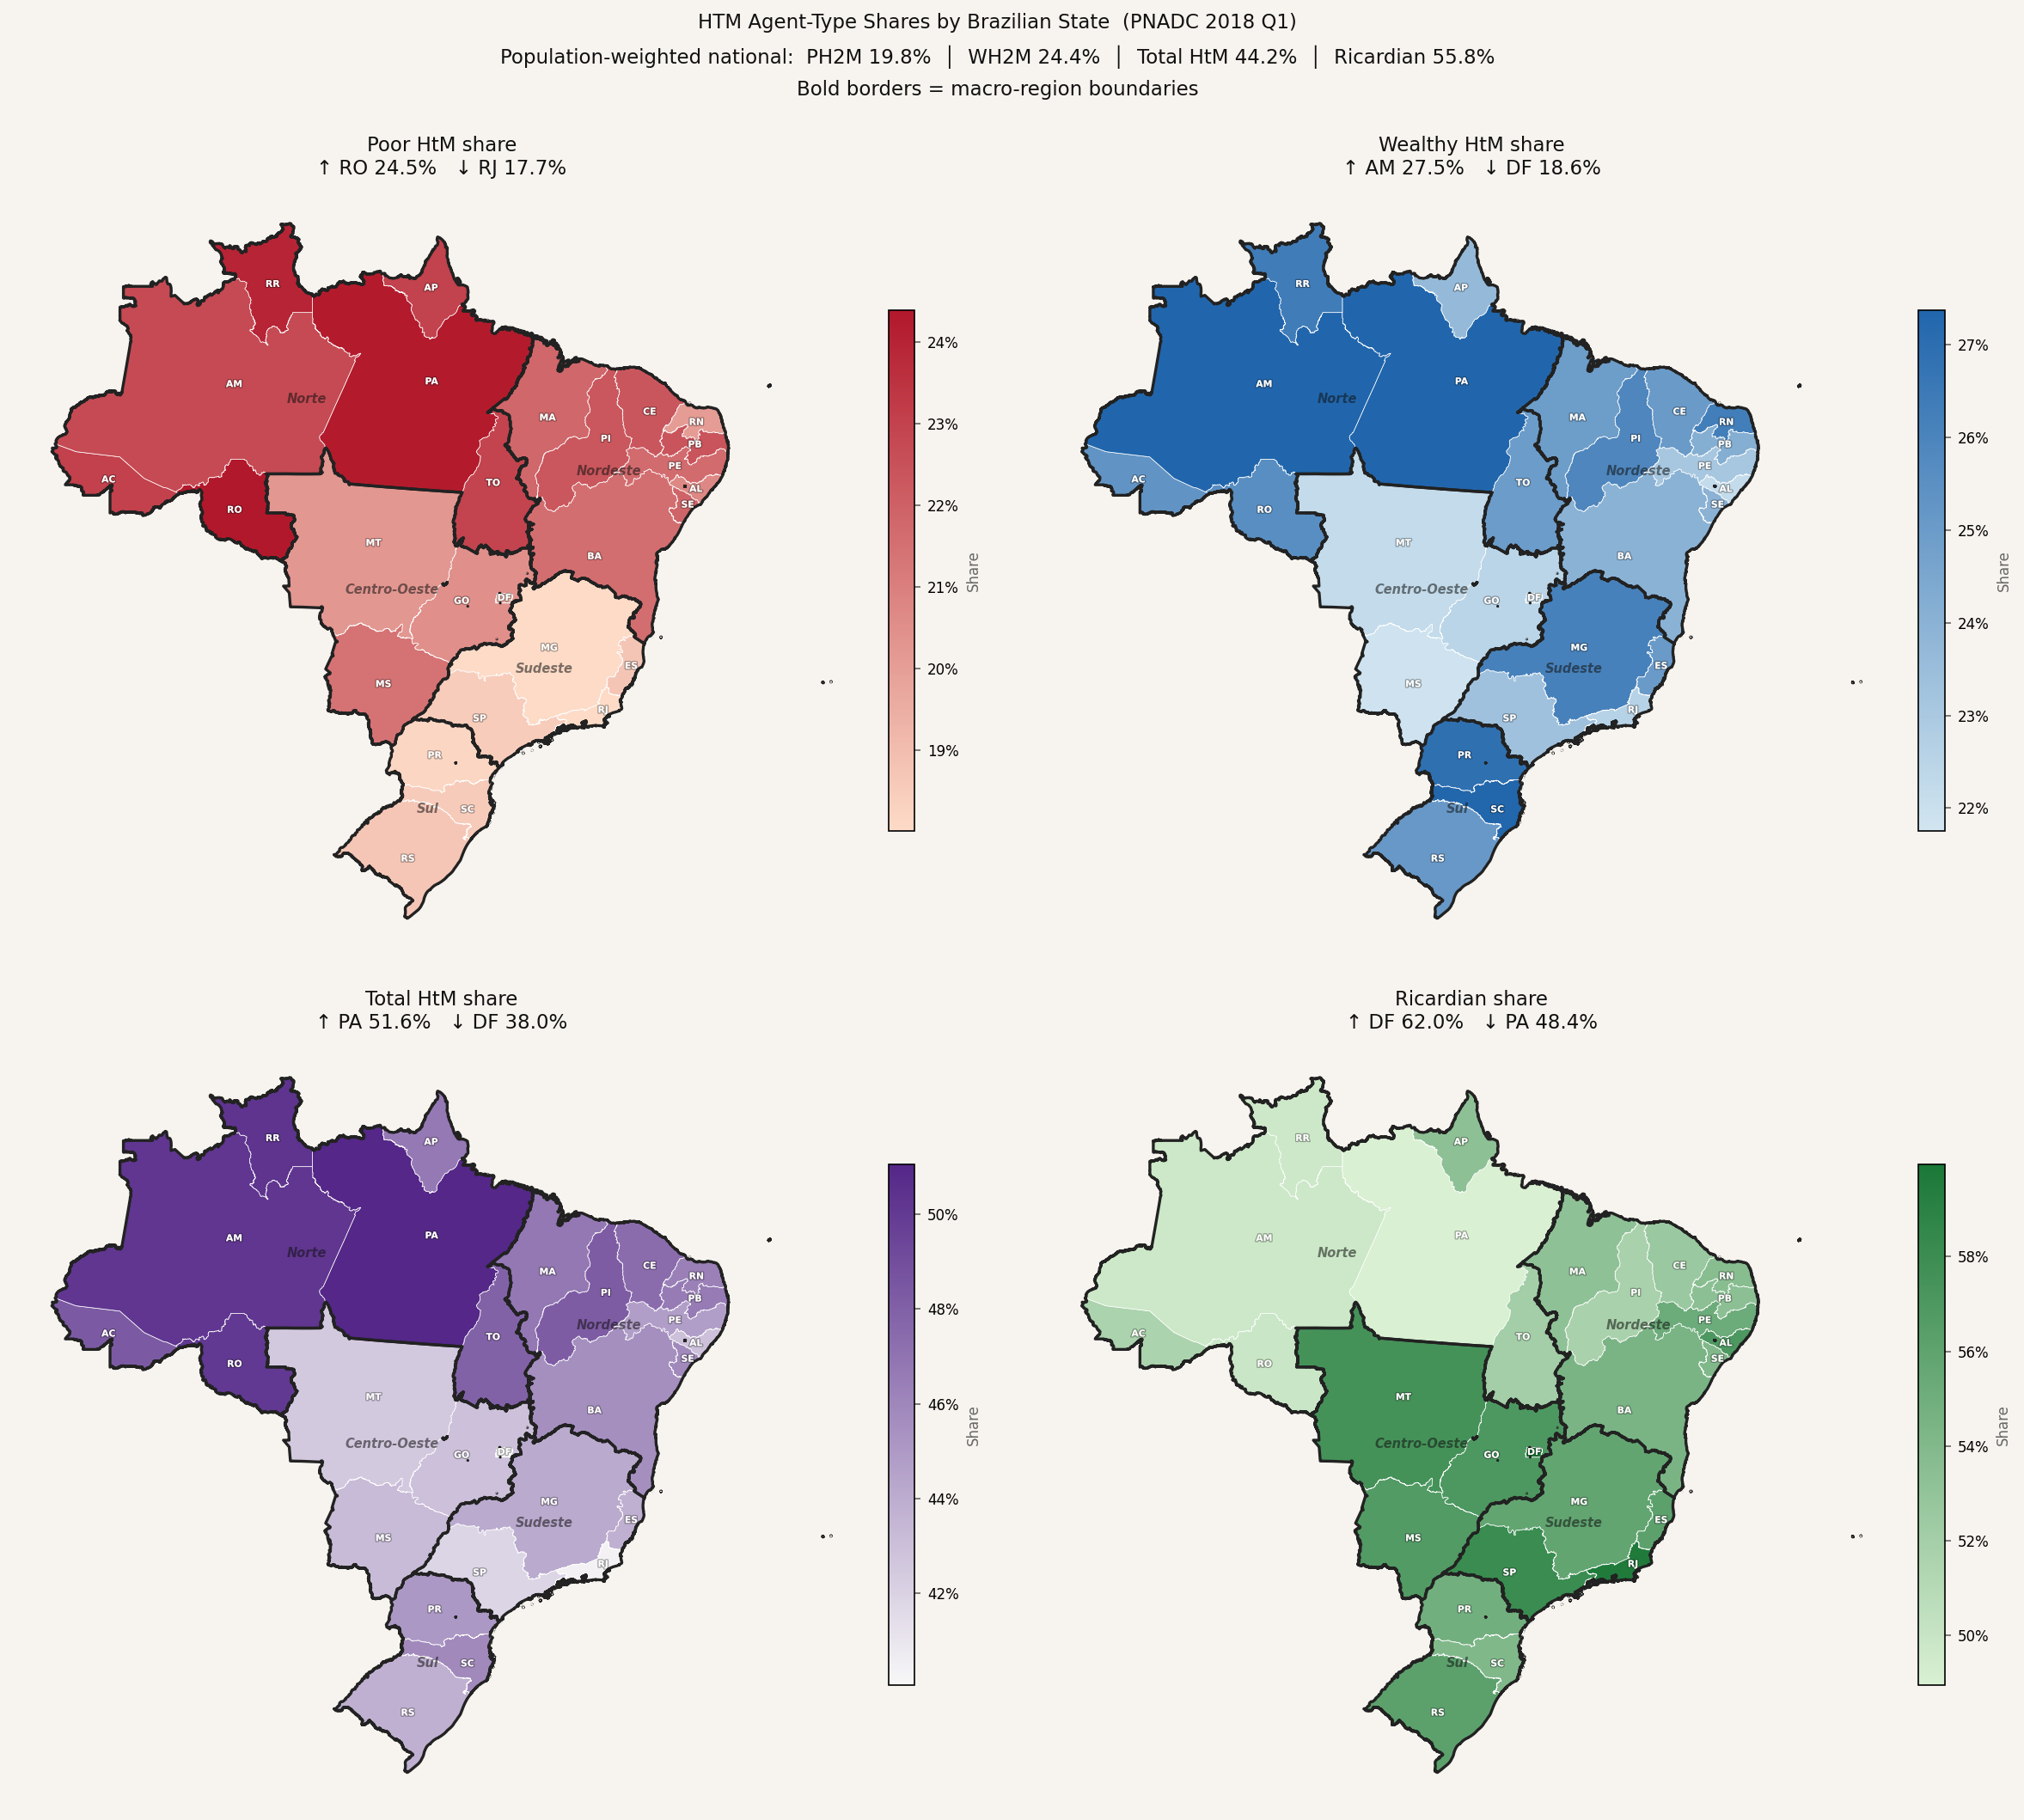
\includegraphics[height=0.75\textheight,keepaspectratio]{Graphs/choropleth_htm_2018Q1.png}
  \end{center}
\end{frame}
\begin{frame}{Choropleth Maps --- 2018 Q2}
  \vspace{-0.5em}
  \begin{center}
    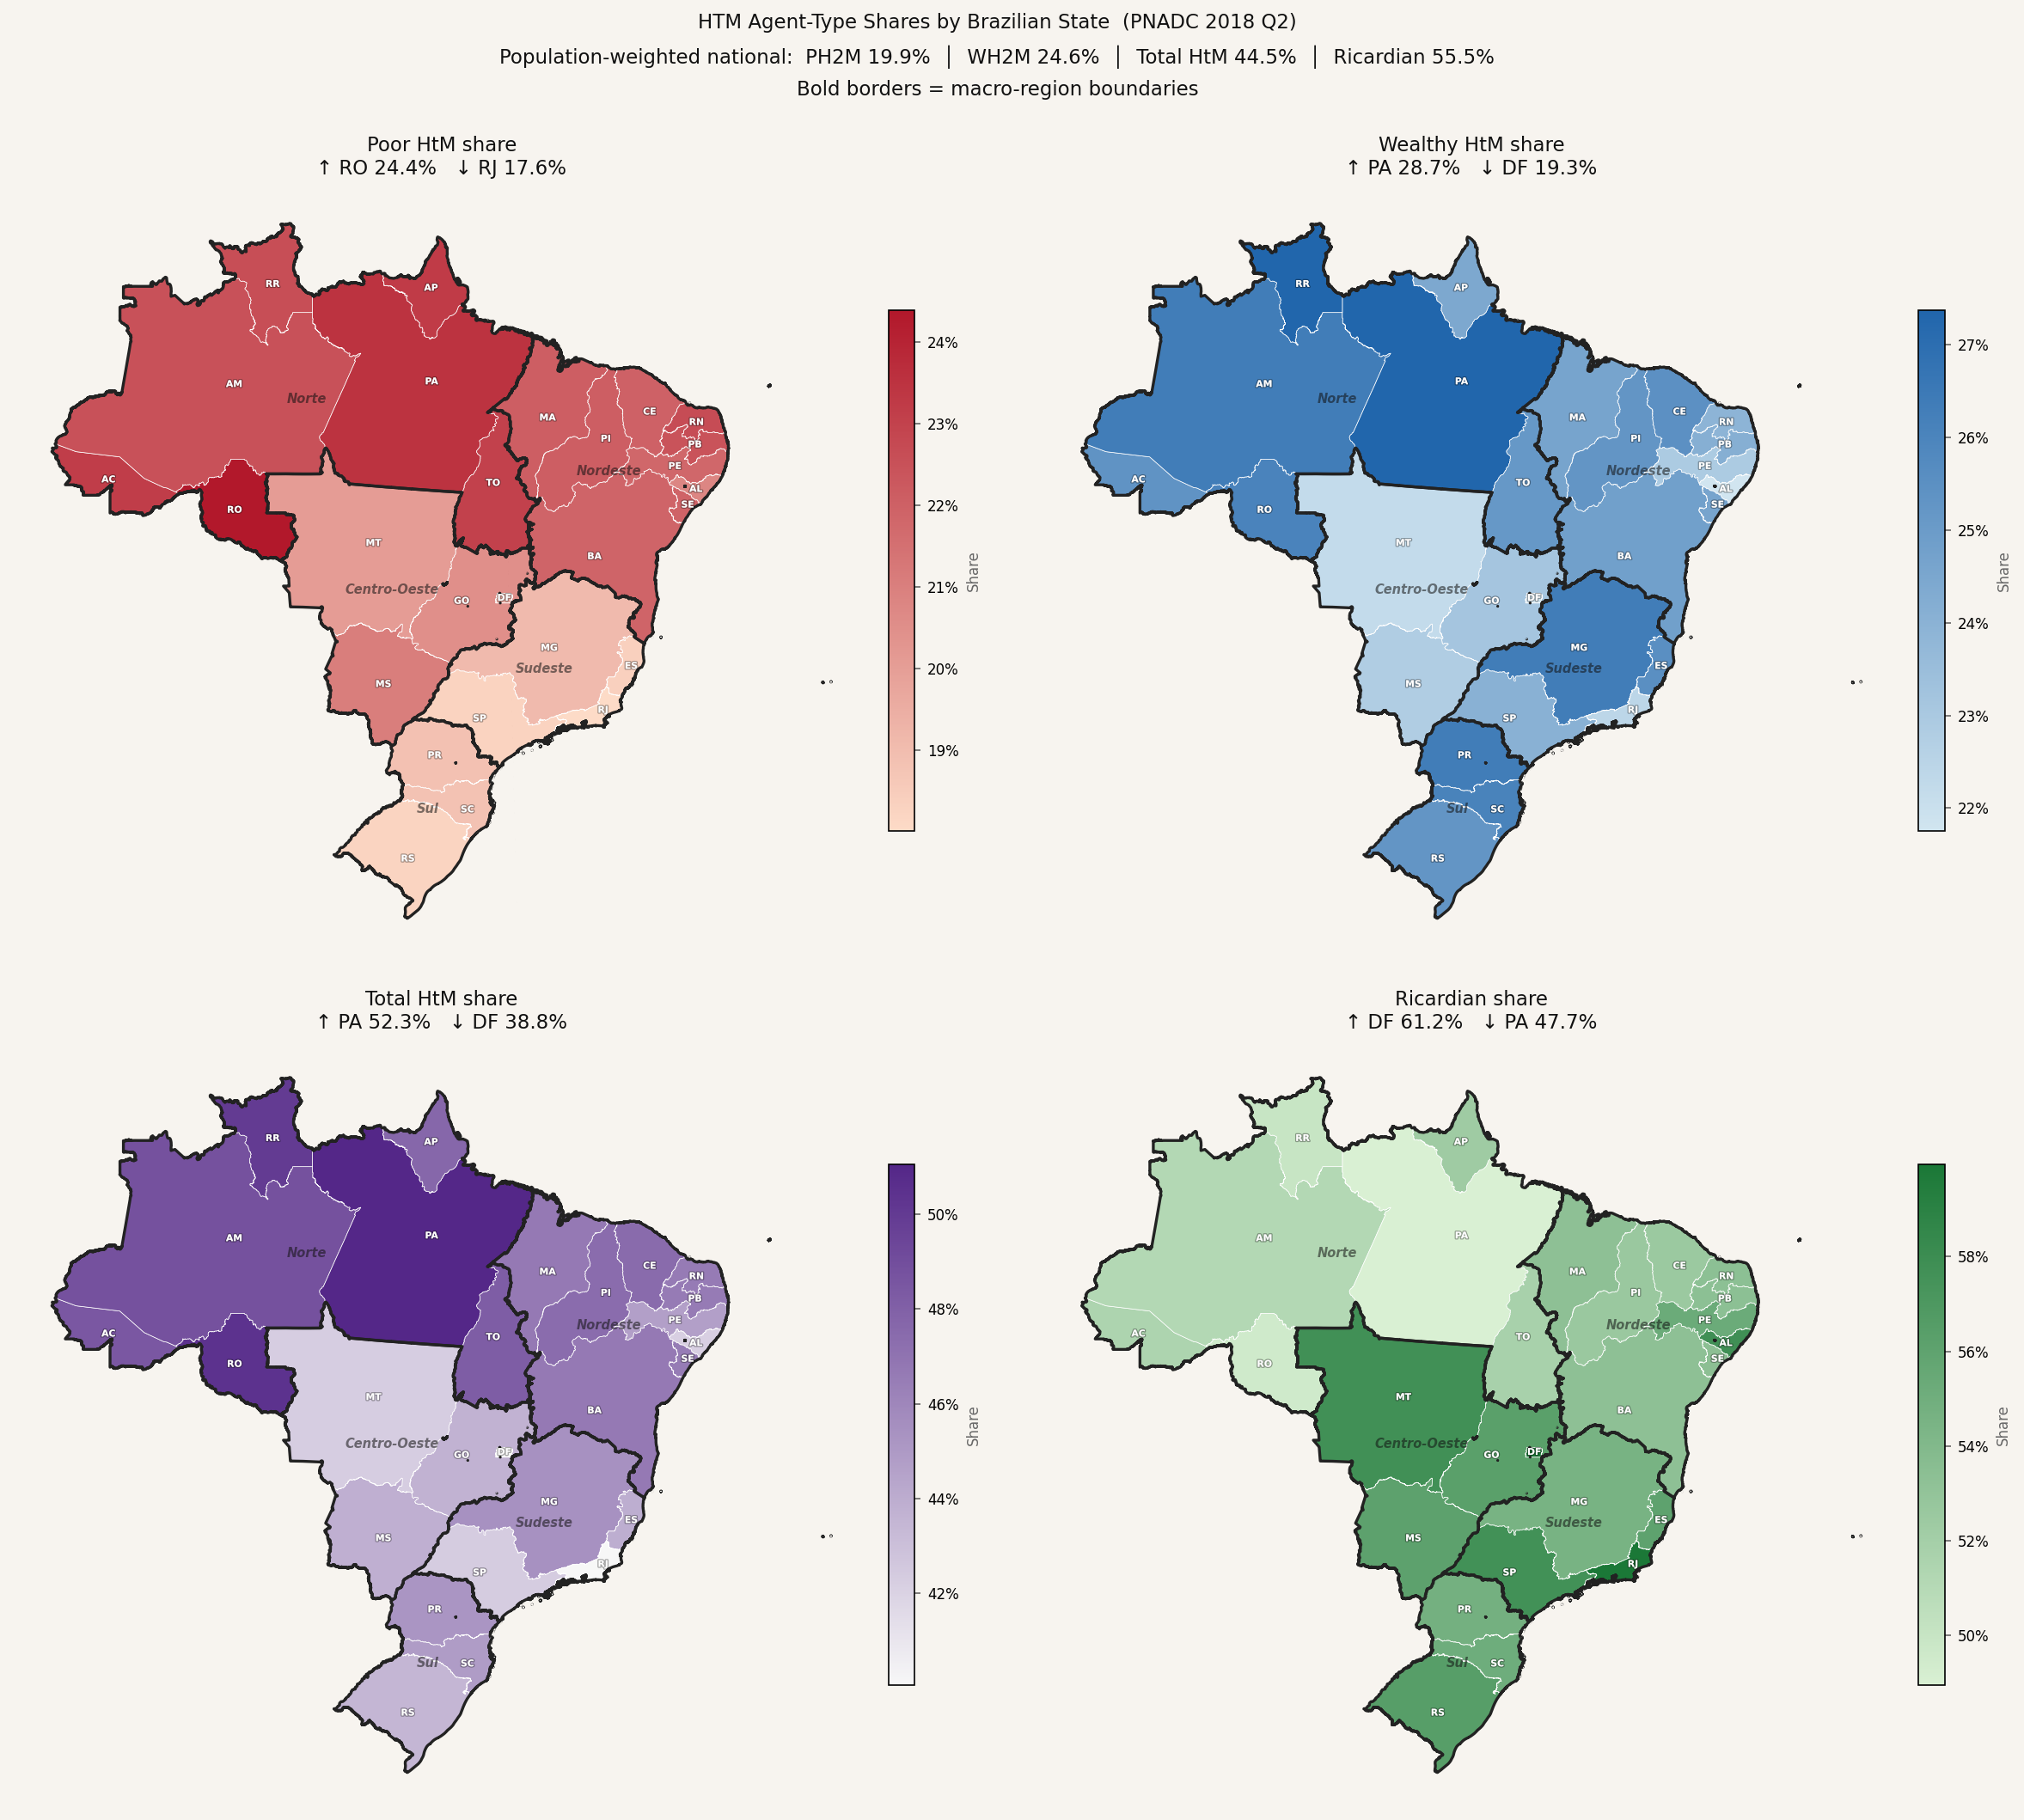
\includegraphics[height=0.75\textheight,keepaspectratio]{Graphs/choropleth_htm_2018Q2.png}
  \end{center}
\end{frame}
\begin{frame}{Choropleth Maps --- 2018 Q3}
  \vspace{-0.5em}
  \begin{center}
    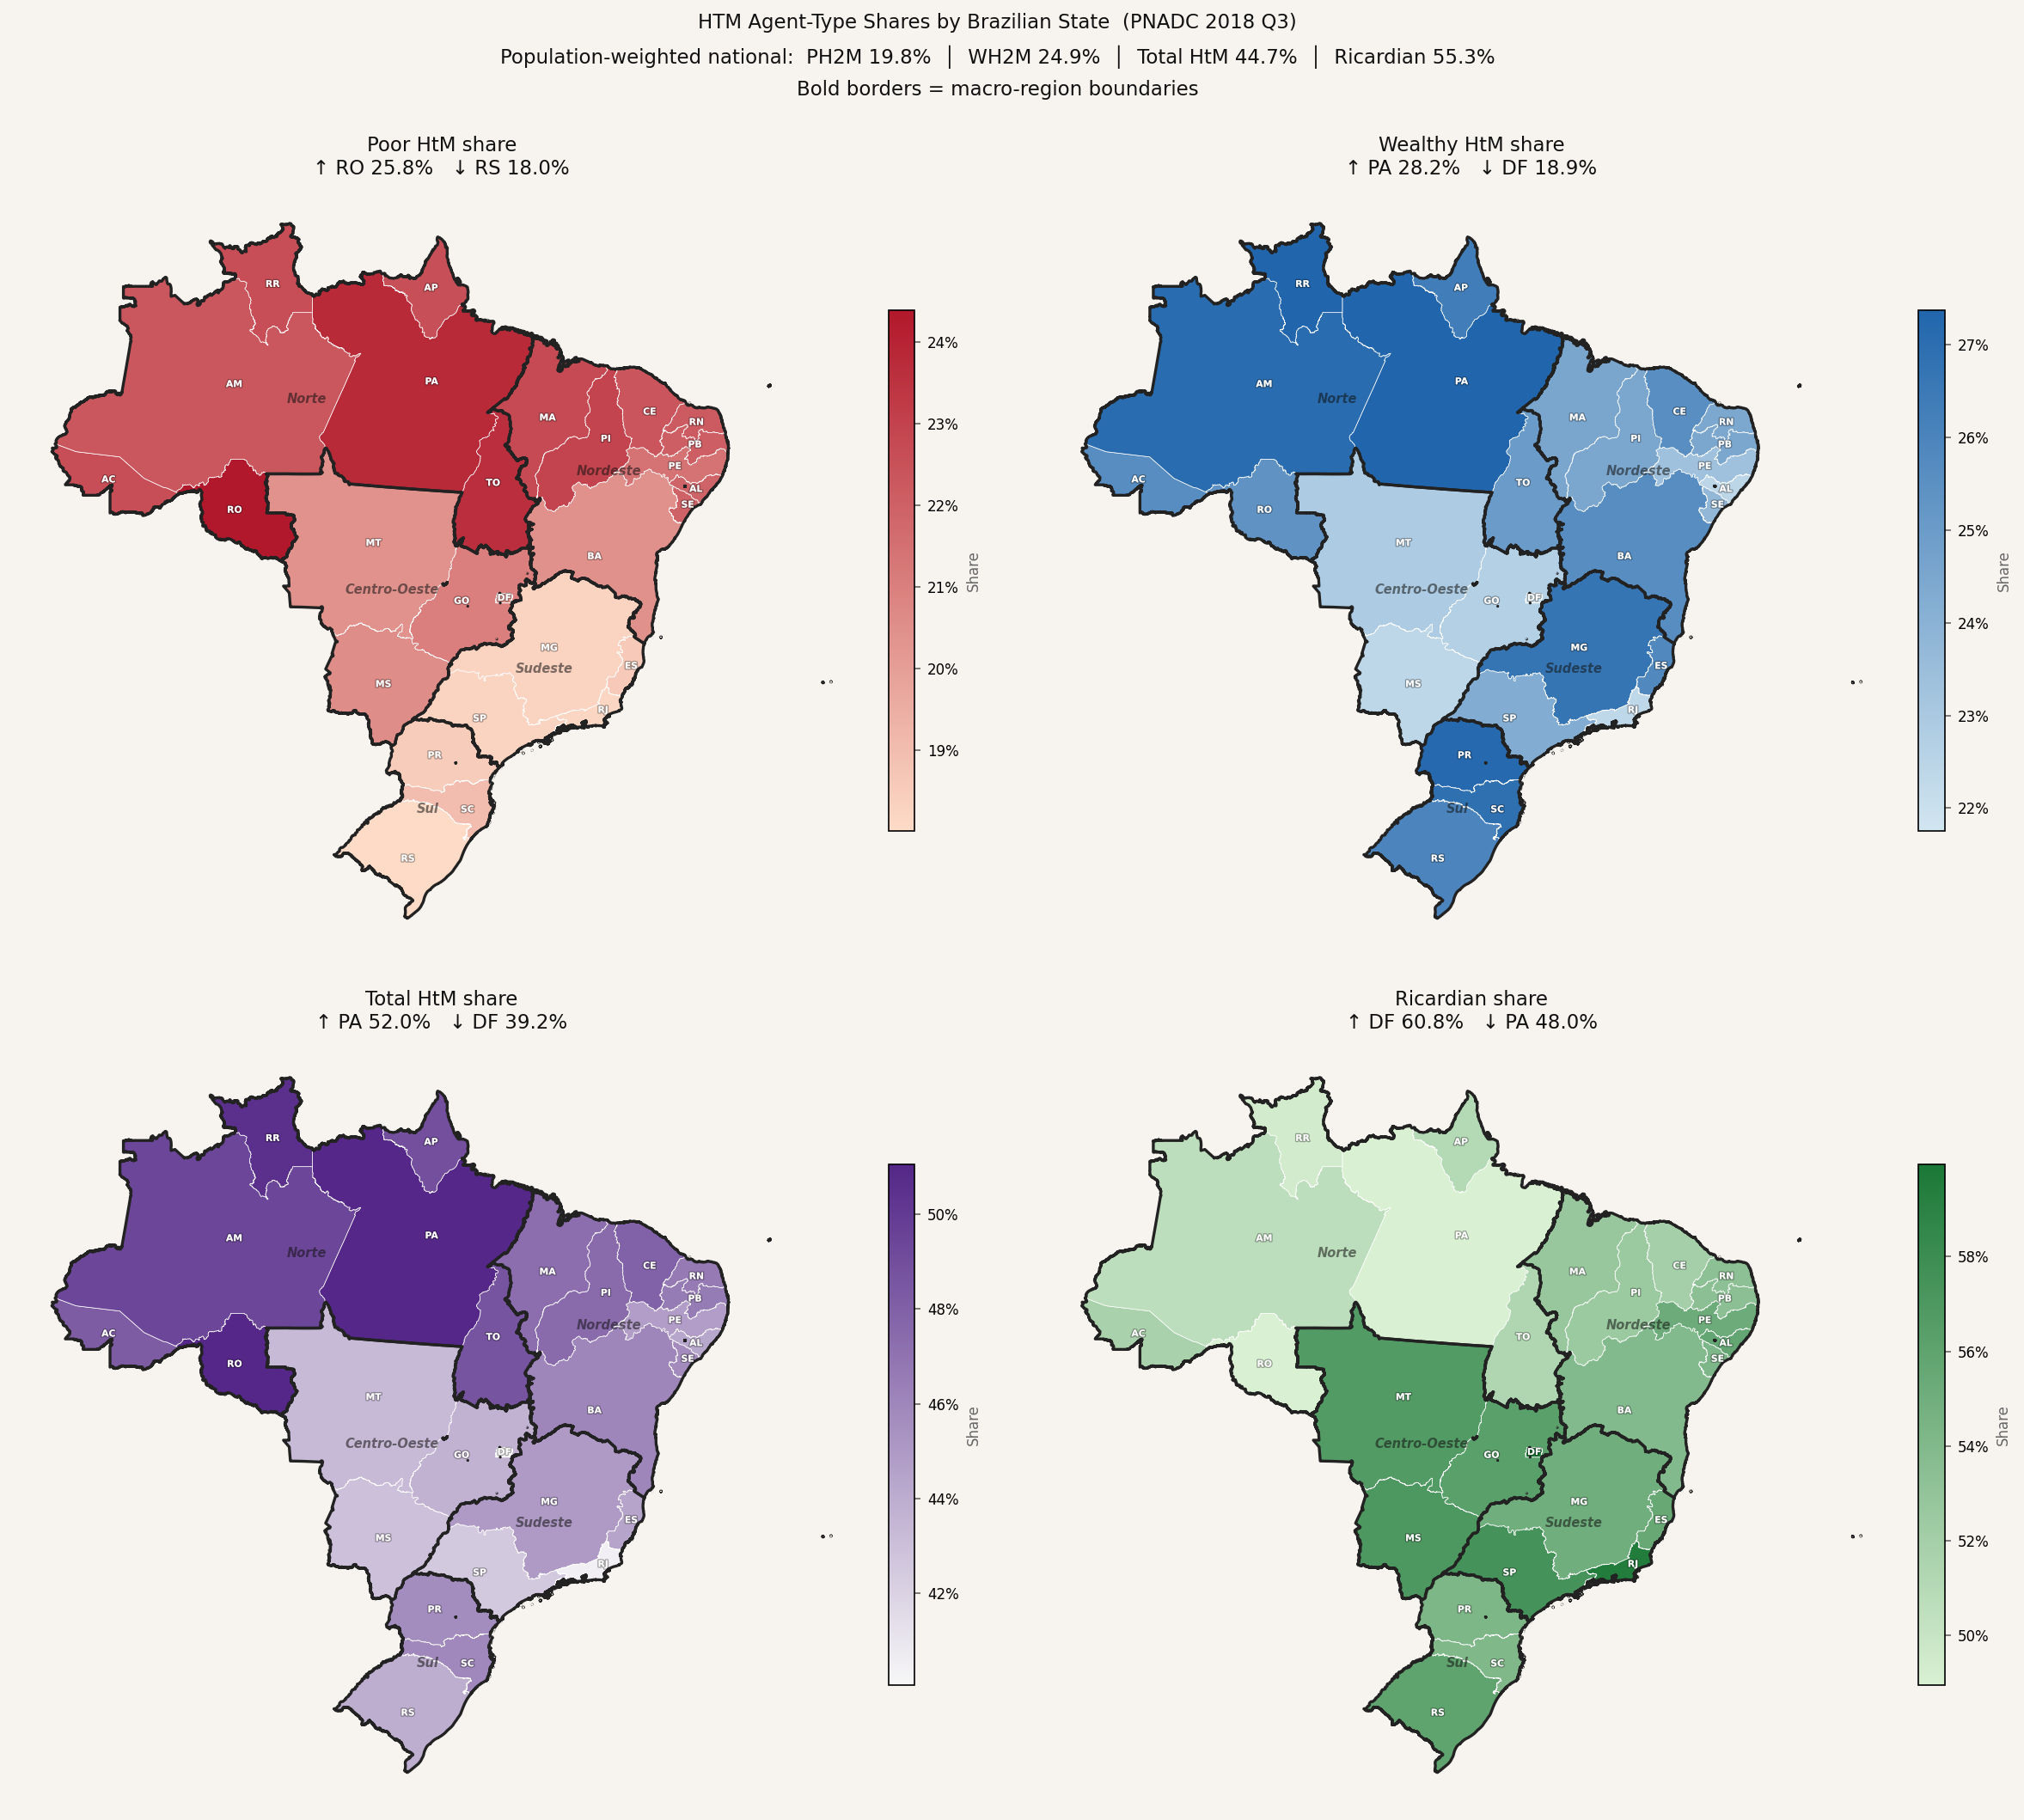
\includegraphics[height=0.75\textheight,keepaspectratio]{Graphs/choropleth_htm_2018Q3.png}
  \end{center}
\end{frame}
\begin{frame}{Choropleth Maps --- 2018 Q4}
  \vspace{-0.5em}
  \begin{center}
    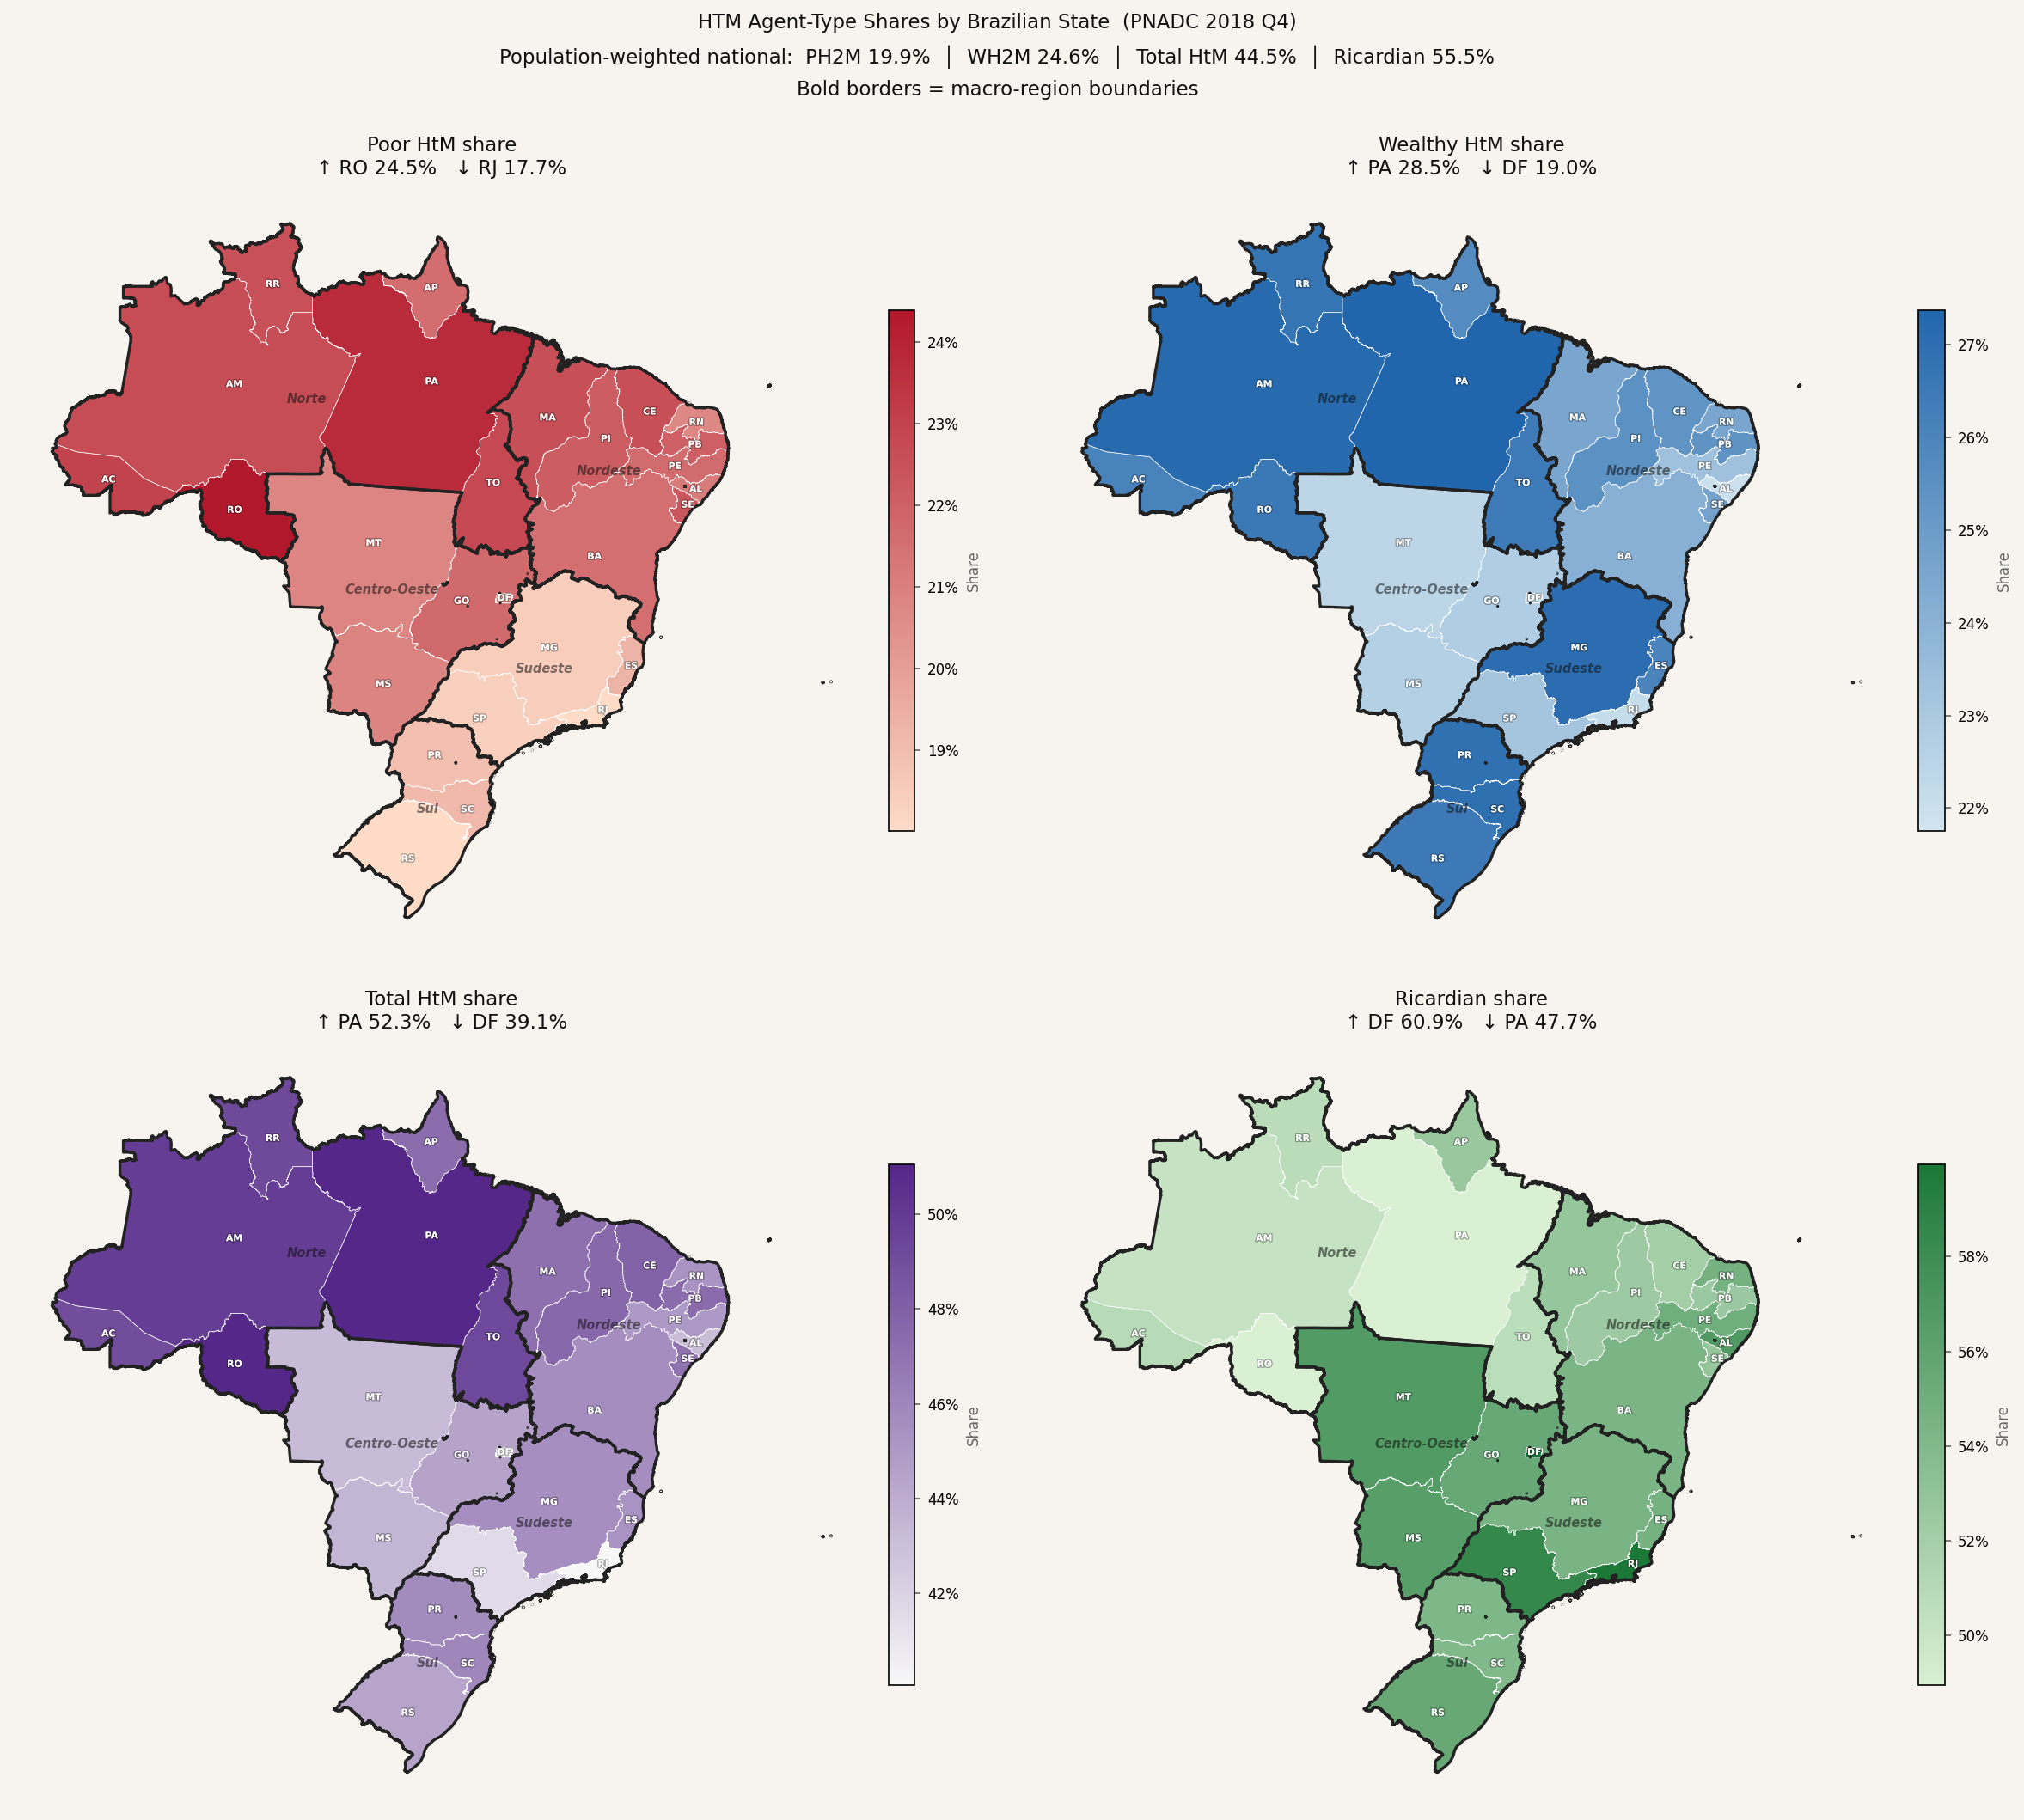
\includegraphics[height=0.75\textheight,keepaspectratio]{Graphs/choropleth_htm_2018Q4.png}
  \end{center}
\end{frame}
\section{Robustness}

\begin{frame}{Robustness}
  $\lambda$ swept 0.25--1.50 in steps of 0.25; other params fixed.
  \vspace{0.5em}
  \textbf{Findings:}
  \begin{itemize}
    \item PH2M highly sensitive: $\lambda - 0.25 \Rightarrow -10$ pp; $\lambda + 0.25 \Rightarrow +18$ pp
    \item WH2M stable: $\pm 3$--4 pp; determined by illiquid threshold
    \item $\lambda = 0.50$: only threshold where all four types sit within literature bands
  \end{itemize}
\end{frame}

\section{Outputs}

\begin{frame}{Output Files}
  \begin{itemize}
    \item \texttt{pof\_bin\_shares.csv} --- demographic bin shares (1,361 bins), Dirichlet smoothing
    \item \texttt{state\_quarter\_htm\_shares.csv} --- 27$\times$8 = 216 rows (weighted)
    \item \texttt{choropleth\_htm\_YYYYQN.png} --- one 4-panel map per quarter (PH2M, WH2M, total HtM, Ricardian)
  \end{itemize}
\end{frame}

\end{document}
